\chapter{Goals and Use Cases}
\label{ch:Goals and Use Cases}

In this chapter, the intended goals of the project and some use cases are being discussed.

\section{Goals}

The goal of the project is to develop a software suite which facilitates inter-operability between MANO frameworks, thereby enabling the management of a network service across a multi-vendor environment. To achieve this, the software suite is divided into 3 individual work packages (WPs), which are initially developed in parallel and are merged later. In the following sections, the individual goals of these work packages are explained in detail.

\subsection{Service Descriptor Translator (SDT)}

In this work package, a translator engine for a NSD is implemented. The Network Function Virtualization Orchestrator (NFVO) is the main orchestration unit of a MANO framework that manages the lifecycle of a network service. One of the main functions of a NFVO is registering a network service, by on-boarding it's NSD to the network service catalog. In a scenario where a network service is to be deployed among two different MANO
frameworks, having their own respective NSD schema, SDT engine would help in translating a NSD schema from one MANO framework to the other framework. 
\subsection{Service Descriptor Splitter (SDS)}

In the production environment, a network service is deployed over a vast geographical region spanning multiple domains. In such scenarios, there is a need to split a network service into smaller network services and deploy it over multiple domains. In this work package, a Service Descriptor Splitter (SDS) is implemented which splits the NSD of a network service. SDS takes NSD as an input that contains all the information elements which can be extracted to generate separate NSDs. In the proposed approach, the service graph is extracted from the input NSD and is split into subgraphs that result in a separate NSD which includes a set of elements such as VNFs, Virtual Links (VLs), forwarding graphs of VNFs etc, according to the specific MANO framework.

\subsection{MANO Adaptor (MA)}

A key component of a MANO framework is Virtualized Infrastructure Manager (VIM),  which helps in assigning the hardware resources to virtual resources. The MANO framework has specific adaptors to communicate with their respective VIMs. For instance, Sonata  (\ref{SecSONATA}) MANO framework has adaptors for OpenStack (\ref{SecOpenStack}) and Kubernetes (\ref{SecKubernetes}). However, when there is a spike in the service request beyond the capabilities of a single MANO instance, multiple MANO instances should be instantiated to balance the load. The goal of this work package is to build an adaptor that facilitates interaction between different instances of MANO frameworks, thereby exposing the underlying MANO framework's interfaces and enabling monitoring of the underlying service states.

Apart from the implementation of MA, the plan is to investigate MANO scalability challenges (refer \ref{wp3manoresearch})

\subsection{Integration Of Work Packages}
In this work package, the SDT, SDS, and MA are integrated. This integration will augment the functionality of the MA in terms of addressing the scalability challenges between instances of different MANO frameworks. It also extends the capabilities of both the SDS and SDT to split a NSD and then deploy a part of it on a different MANO framework. All these individual modules are planned to be implemented as microservices and are integrated keeping their individuality intact. 
\begin{figure} [h]
	\centering
	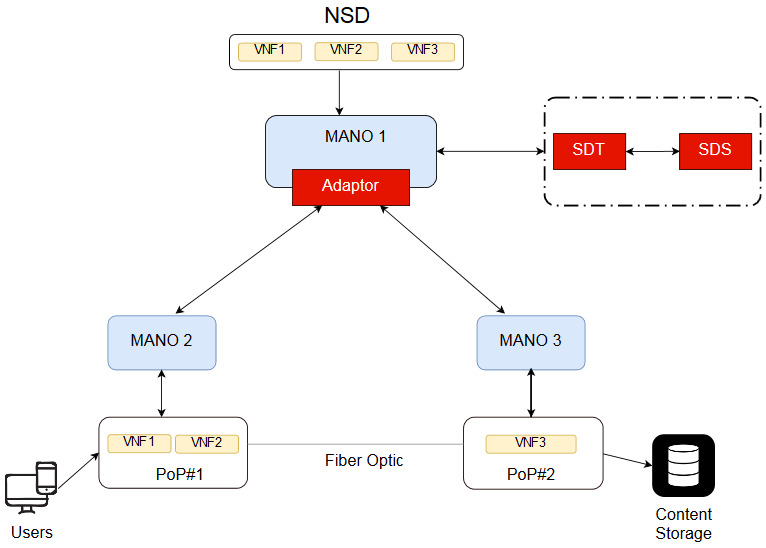
\includegraphics[width=0.8\linewidth]{figures/StructureIntegrated1}
	\caption{This figure visualizes the structure of the software suite.}
	\label{fig:structureintegrated}
\end{figure}

\section{Use Cases}

\subsection{Cross-MANO Framework Interaction}
The MANO frameworks used by every network service provider varies from one another. The software suite with the help of SDT and SDS enables the deployment of network services across different frameworks.

For instance: Consider two network service Operators using different MANO frameworks. One of them uses Sonata framework \cite{draxler2017sonata} and another operator uses OSM framework \cite{ersue2013etsi}. These frameworks have different NSD schemata(refer \ref{SecSONATA} and \ref{SecOSM}). NSD schemata contain VNFs, virtual links, and VNF forwarding graphs and also describes the deployment of a network service. By using a translator and splitter, these NSD schemata can be translated and split into a framework-specific schema. With this, operators can deploy and manage network services across different MANO implementations.

\subsection{Hierarchical Orchestration}
By using MA, dynamic instantiation of multiple MANO instances and inter-operability between different MANO frameworks can be achieved. The operator will be able to handle the resources in an efficient manner, as one MANO framework can manage a limited number of service requests, operators can explore options to include additional MANO instances under the existing MANO instance to mitigate the traffic load on a single instance. The resources can be provisioned based on the number of requests. This helps the operator in extending their profitability.

\textbf{Actors} : The Network Service Providers who would use features of SCrAMbLE.

\begin{figure} [h]
	\centering
	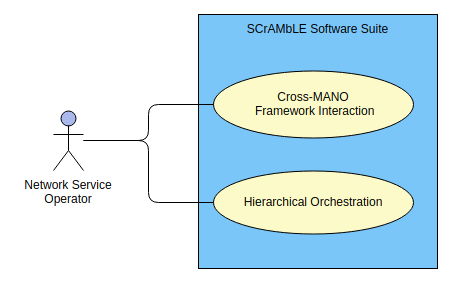
\includegraphics[width=0.9\linewidth]{figures/use-case}
	\caption{Use Case Diagram}
	\label{fig:use-case}
\end{figure}





